\documentclass[11pt,a4paper]{article}

\usepackage[margin=1.1in]{geometry}
\usepackage{amsmath,amssymb}
\usepackage[hidelinks]{hyperref}
\usepackage{enumitem}
\usepackage{tikz}
\usepackage{xcolor}
\usepackage{titlesec}
\usepackage[expansion=false]{microtype}
\usetikzlibrary{arrows.meta,positioning,fit,backgrounds,shapes.geometric}

\definecolor{abstrcol}{HTML}{2C5F8A}
\definecolor{numcol}{HTML}{D4850A}
\definecolor{boxbg}{HTML}{F5F5F5}

\titleformat{\section}{\Large\bfseries\color{abstrcol}}{}{0em}{}
\titlespacing{\section}{0pt}{1.4em}{0.5em}

\newcommand{\creed}[1]{\item \textbf{#1}}

\title{\textbf{Git for Science}\\[0.3em]
       \large\normalfont A substrate for reproducible, compounding scientific knowledge}
\author{G. Barbalinardo\\\small University of California, Davis}
\date{\today}

\begin{document}
\maketitle
\thispagestyle{empty}

% ---- Hook ----
\noindent
Git did not just store files. It stored the \emph{repository}: a structured,
content-addressed object with identity and lineage, of which the working files
are one view. That object is why merging, provenance, and collaboration became
mechanical, and why a planet's worth of code could accumulate in one shared form.
Science is still pre-git. We ship the paper, the printout of a result, and throw
the object away. This is an attempt to store the object: what a result
\emph{is} (a typed physical quantity, its formula, its lineage, and the code that
produced it as one representation of it), so that results become reproducible by
construction, knowledge compounds instead of evaporating, and an AI agent has a
semantic place to act.

% ---- Creed ----
\section*{\color{abstrcol}The creed}
\begin{enumerate}[leftmargin=1.4em, itemsep=0.35em]
  \creed{The unit of scientific knowledge is meaning, not text.}
  \creed{Physics is the invariant. A code is one representation of it.}
  \creed{A scientific result is a structured object with identity and lineage, not a number in a table.}
  \creed{A result you cannot re-run is a claim, not yet knowledge.}
  \creed{Units, gauge, and lineage are part of a result, not footnotes to it.}
  \creed{Knowledge should compound, not evaporate into scripts.}
  \creed{Correctness should be structural, checked by the substrate, not re-derived by trust.}
  \creed{Verification must scale with compute, not with reviewers.}
  \creed{The native substrate for scientific AI is semantic, not token text.}
\end{enumerate}

\section{The problem: science that does not accumulate}

Computational materials science is a Tower of Babel. A single physical quantity,
say the lattice thermal conductivity of a crystal, is computed by a dozen codes:
kaldo, phono3py, ShengBTE, LAMMPS, VASP, Quantum ESPRESSO. Each has its own input
formats, its own unit conventions, its own gauge and basis choices, and its own
unspoken assumptions about what was held fixed. The physics is the same. The codes
never quite agree, and deciding whether two of them \emph{should} agree is itself
expert work.

That work does not accumulate. Reconciling two calculations is artisanal, done by
a handful of people who carry the conventions in their heads, and most published
computational results are effectively irreproducible because the real workflow
lives in tribal knowledge and one-off scripts rather than in the paper. The paper
is the tarball we email. Once it is sent, the object that produced it is gone.

\section{The diagnosis: meaning is implicit}

The reason the codes do not agree mechanically is that their meaning is implicit.
Scientific knowledge today lives in three forms, and each loses something. Prose,
in papers, carries rich meaning but does not run. Code runs, but its meaning is
entangled with implementation: the physics is mixed in with array layouts, loop
orders, and file formats. Data is numbers stripped of their provenance. None of
the three carries meaning that is at once machine-checkable and runnable.

So the physics is never stored directly. It is buried inside whichever artifact
happened to carry it, and recovering it, deciding what a given number actually
claims, is left to the reader. What cannot be recovered mechanically cannot be
checked mechanically, and so it cannot accumulate.

\section{The bet: store the physics, not the printout}

The move is to store the object. A result becomes a typed quantity, thermal
conductivity or a phonon frequency or a heat capacity, declared as what it is. The
formula that produces it rides on the edge that produces it, written symbolically
rather than implied by code, and the quantity carries its lineage, the ordered
chain of operations behind it, along with its units and gauge. A code is then no
longer the result; it is one \emph{representation} of it, a projection of a single
shared operator layer into one discretization and one set of conventions.

Every representation factors through that shared layer, never code to code. That
is what makes reconciliation mechanical: two codes that computed the same
observable are two projections of one object, so comparing them is a structural
operation on the graph rather than a feat of expert translation. It is merge, for
science.

\begin{figure}[h]
\centering
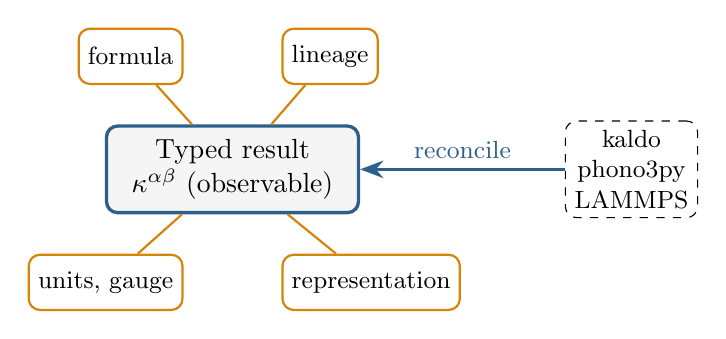
\begin{tikzpicture}[
  node distance=6mm,
  obj/.style={draw=abstrcol, very thick, rounded corners, fill=boxbg,
              minimum width=3.2cm, minimum height=1.1cm, align=center},
  tag/.style={draw=numcol, thick, rounded corners, fill=white,
              font=\small, align=center, minimum height=0.7cm},
  rep/.style={draw, dashed, rounded corners, font=\small, align=center}]

  \node[obj] (q) {Typed result\\$\kappa^{\alpha\beta}$ (observable)};
  \node[tag, above left=5mm and -1cm of q] (f) {formula};
  \node[tag, above right=5mm and -1cm of q] (l) {lineage};
  \node[tag, below left=5mm and -1cm of q] (u) {units, gauge};
  \node[tag, below right=5mm and -1cm of q] (p) {representation};
  \foreach \n in {f,l,u,p} \draw[numcol, thick] (q) -- (\n);

  \node[rep, right=2.6cm of q] (codes) {kaldo\\phono3py\\LAMMPS};
  \draw[->, >=Stealth, abstrcol, very thick] (codes) -- node[above, font=\small]{reconcile} (q);
\end{tikzpicture}
\caption{A scientific result as a structured object: a typed quantity carrying its
formula, lineage, units and gauge, with each code a representation that reconciles
into it at the observable. Merge, for science.}
\end{figure}

This is the same decision git made. A commit is identified by its content and its
parents; a result here is identified by its type and its lineage. Git won on its
object model, the blobs and trees and commits, not on its interface, and the
contribution here is the analogous object model for a scientific result. Getting
that object right is the whole game.

One difference is worth stating plainly, because it is where the real work lives.
Code is discrete and born digital, while a scientific result carries approximation,
continuous quantities, and gauge freedom: a per-mode lifetime depends on a basis
choice no two codes share, even though the conductivity it sums to does not. That
is why the object is typed, why units travel with it, and why the layer separates
\emph{observable} quantities, which must agree across codes, from
representation-dependent scaffolding, which need not. Defining what is allowed to
differ is as much of the design as defining what must match. The project already
ingests a \emph{code} this way; the vision is to ingest a \emph{paper} the same
way, turning its claims into objects the substrate can hold, re-run, and check.

\end{document}
